\addcontentsline{toc}{chapter}{Разработка метода тактильного очувствления}

\textbf{\underline{Четвертая глава}} раскрывает детали определения профиля опорной поверхности, на основе информации о точках её касания ногами робота и внутренних датчиков, характеризующих механическое состояние аппарата. Вторая часть главы показывает определение с помощью робота физико-механических свойств опорной поверхности:
жесткости, упругости и пластичности.

\textbf{Первая задача:} с помощью ощупывания роботом поверхности получить плотное облако точек и полигональную сетку. 

Метод основан на триангуляции Делоне с использованием альфа формы. Идея решения: решив задачу локализации точки касания ногой робота опорной поверхности, получить облако точек следовой дорожки. Далее, необходимо очистить шумное облако точек и его усреднить с помощью Voxel Grid. Применив триангуляцию Делоне для вогнутых оболочек \pic{fig:exp_concave_}, получается полигональная сетка. На ее основе можно сгенерировать новые точки из полигональной сетки с нужным разрешением. Подразумевается, что расстояние между ногами робота мало относительно размеров поверхности, следовательно, поверхность между ногами считается плоскостью.

Входными данными является следовая дорожка, в виде облака точек. Выходными --- полигональная сетка и плотное облако точек. Допустимая точность: 0.1 м, оценки Cloud2Cloud и Cloud2Mesh.

Апробация метода проводилась в симуляции (Рис. \ref{fig:unsolvable_case}) и натурно \pic{fig:real_exp_map_creation}.



% \begin{figure}[H]
%     \centering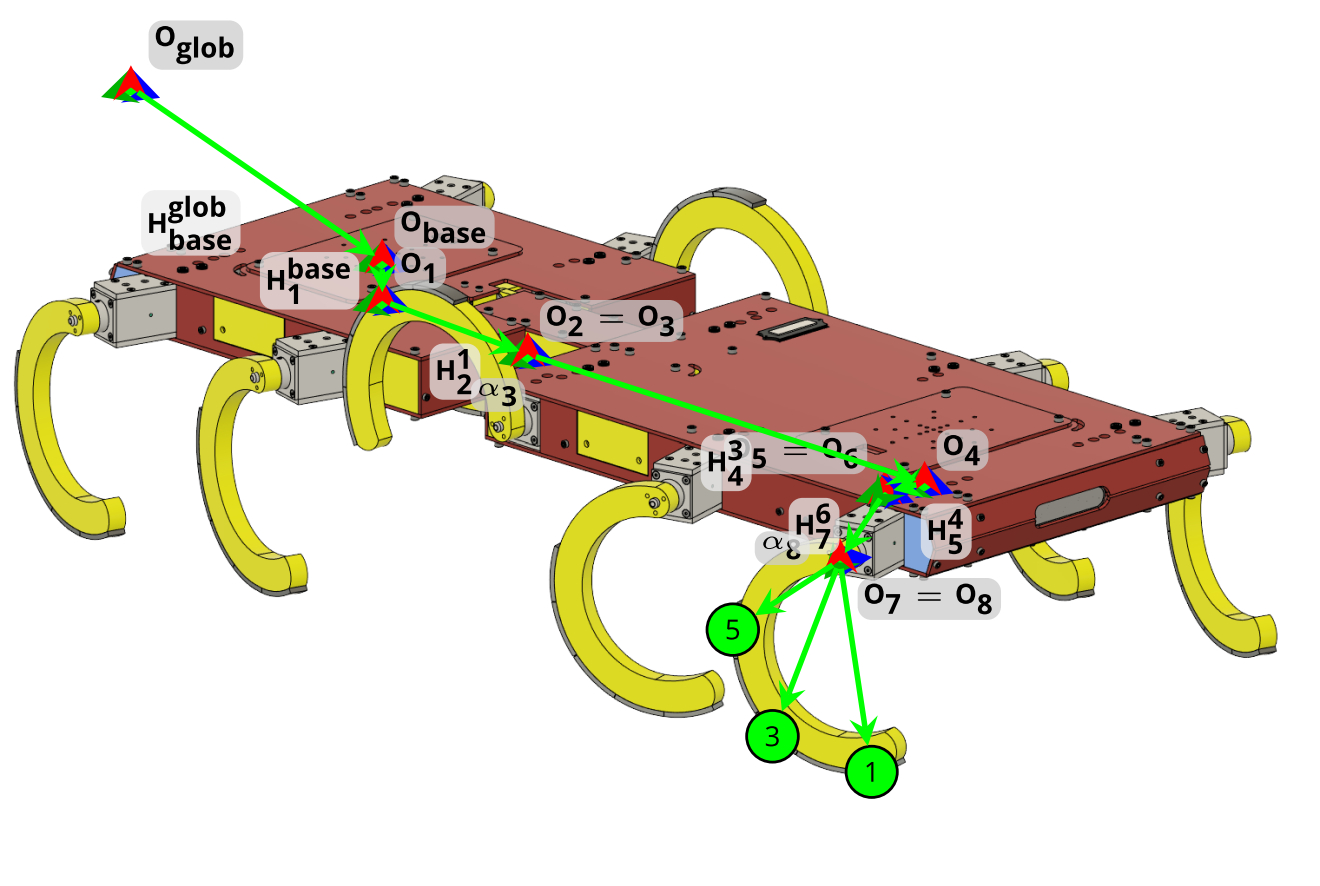
\includegraphics[height=4cm,width=1\textwidth,keepaspectratio]{tikz_exp/tikz_pictures8.png}
%     \caption{Кинематическая схема для определения точки касания опорной поверхности роботом}
%     \label{fig:StriRus_10_legs_15_angle_v4.png}
% \end{figure}

% \begin{multline}
%     \label{eq:forw_kin}
%         H_{leg}^{glob} = H(x_{glob},y_{glob},z_{glob},\alpha_{glob},\beta_{glob},\gamma_{glob})T_z(l_1)\\ T_x(l_2)R_y(\alpha_3)T_x(l_4)T_y(l_5)R_z(-15^{\circ})T_y(l_7)R_y(\alpha_8)
% \end{multline}
% Где каждая матрица представляет собой матрицу однородного преобразования, через $R_i$ обозначены однородные матрицы поворота, относительно соответствующей оси, $T_i$ --- однородную матрицу перемещения.

\begin{figure}[h]
    \begin{subfigure}[t]{0.32\textwidth}
        \centering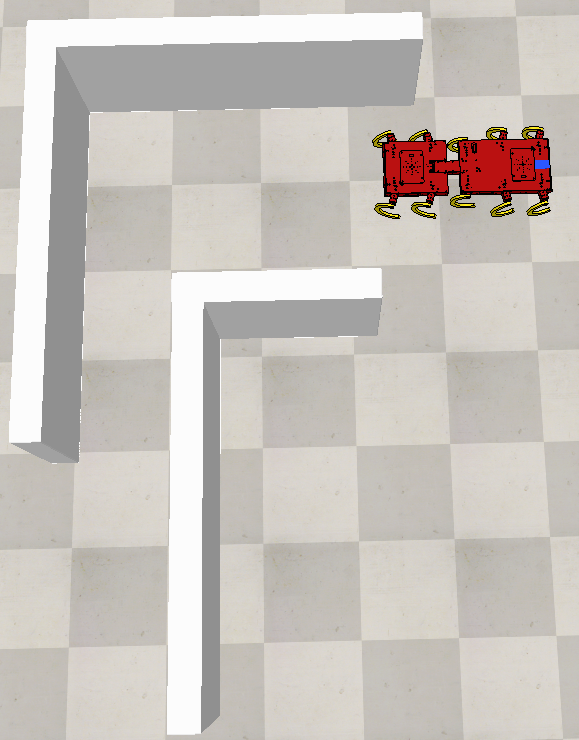
\includegraphics[height=4cm,width=1\textwidth,keepaspectratio]{convex_terr.png}
        \caption{Пример поля}
        \label{fig:convex_terr.png}
    \end{subfigure}
    \begin{subfigure}[t]{0.32\textwidth}
        \centering
        \begin{tikzpicture}
            % Include the image in a node
            \node [above right, inner sep=0] (image) at (0,0)
            {\centering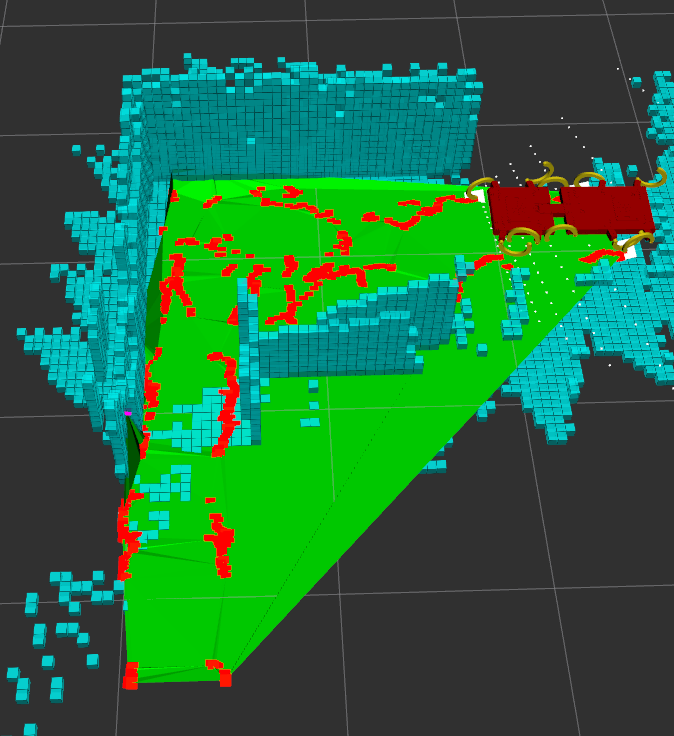
\includegraphics[height=4cm,width=1\textwidth,keepaspectratio]{conv_convex.png}};
            % Create scope with normalized axes
            \begin{scope}[
                x={($ 0.1*(image.south east)$)},
                y={($ 0.1*(image.north west)$)}]
            % Labels
            \draw[stealth-, very thick,green] (5.2,3.5) -- ++(0,-1)
            node[rounded corners=3pt,right,black,fill=white]{\tiny Полученная сетка};

            \draw[stealth-, very thick,green] (5.5,5.5) -- (6.4,4)
            node[rounded corners=3pt,right,black,fill=white]{\tiny Данные лидара};

            \draw[stealth-, very thick,green] (3.4,0.8) -- (5,1);
            \draw[stealth-, very thick,green] (3.4,2.6) -- (5,1)
            node[rounded corners=3pt,right,black,fill=white]{\tiny Следовая дорожка};
        \end{scope}
        \end{tikzpicture}
        \caption{Выпуклая оболочка}
        \label{fig:conv_convex.png}
    \end{subfigure}
    \begin{subfigure}[t]{0.32\textwidth}
        \centering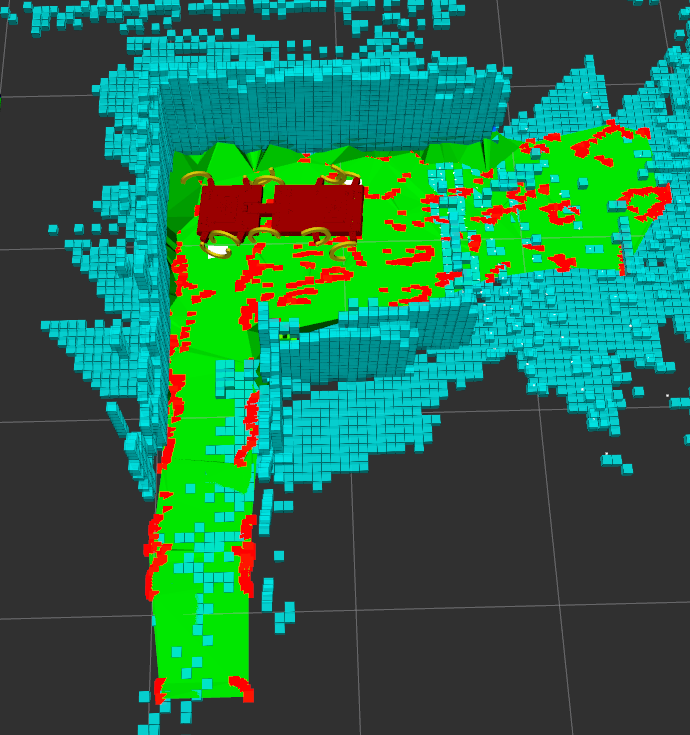
\includegraphics[height=4cm,width=1\textwidth,keepaspectratio]{conv_concave.png}
        \caption{Вогнутая оболочка}
        \label{fig:conv_concave.png}
    \end{subfigure}

    \caption{Объяснение необходимости модификации алгоритма Делоне}
    \label{fig:exp_concave_}
\end{figure}

\begin{figure}[ht!]
    \begin{subfigure}[t]{0.49\textwidth}
            \centering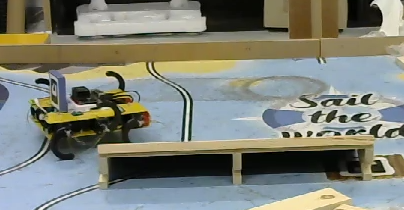
\includegraphics[height=6cm,width=1\textwidth,keepaspectratio]{real_robot_mesh_video_preview.png}
        \caption{Робот проходит препятствие}
        \label{fig:real_robot_mesh_video_preview.png}
    \end{subfigure}
    \begin{subfigure}[t]{0.49\textwidth}
        \centering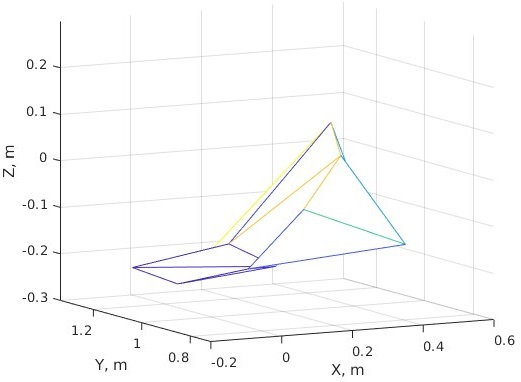
\includegraphics[height=3cm,width=1\textwidth,keepaspectratio]{real_mesh.jpg}
        \caption{Полученная полигональная сетка}
        \label{fig:real_mesh.jpg}
    \end{subfigure}
    \caption{Пример натурного эксперимента}
    \label{fig:real_exp_map_creation}
\end{figure}

Как итог, среднеквадратичная ошибка для C2C метрики была в среднем равна 5 см. А для C2M 1 см. В натурном эксперименте по метрике C2C --- 8 см.

\textbf{Вторая задача} это определение процентного соотношения твердых, упругих и пластичных свойств пройденной поверхности с помощью машинного обучения, метода опорных векторов (SVM). 

Алгоритм решения следующий. Создается установка для обучения \pic{fig:s_shape_leg/s_leg_setup.JPG}. Происходит обучение --- робот ходит по различным типам поверхностей фиксированное количество касаний поверхности с постоянной угловой скоростью. Модель обучается на 80 \% данных с помощью ядра на основе функции Пирсона VII  \eqref{eq:PUK}. Тестирование происходит на оставшихся 20 \%, используются метрики меткости, точности, полноты и F1-счета. Входными данными являются данные с внутренних датчиков сенсора \pic{fig:example_input}.

% В качестве причин выбора таких входных данных можно отметить следующие. Видно различное поведение сенсоров в зависимости от типа поверхности \pic{fig:s_shape_leg/TaxelIndForce_full.png}. Зависимость средней линейной скорости движения ноги на разных поверхностях при различных угловых скоростях \pic{fig:s_shape_leg/avg_lin_vel_rev_min.png}. 

\begin{align}
    \label{eq:PUK}
    K(x, y) = (1 + ((||x - y||^2)/\sigma^2)^\omega)^{(-1/\omega)}
\end{align}
Где $x$, $y$ --- векторы во входном пространстве, $||x - y|||$ обозначает евклидово расстояние между $x$ и $y$, $\sigma$ --- масштабный параметр, определяющий <<разброс>> ядра, $\omega$ --- параметр, влияющий на форму границы принятия решения.

\begin{figure}[h]
    \begin{subfigure}{0.54\textwidth}
        \centering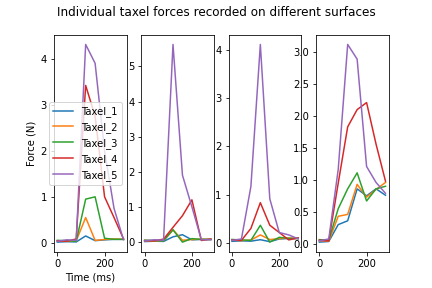
\includegraphics[height=3cm,width=1\textwidth,keepaspectratio]{s_shape_leg/TaxelIndForce.png}
        \caption{Запись активных датчиков силы на разных поверхностях}
        \label{fig:s_shape_leg/TaxelIndForce_full.png}
    \end{subfigure}
    \begin{subfigure}{0.45\textwidth}
        \centering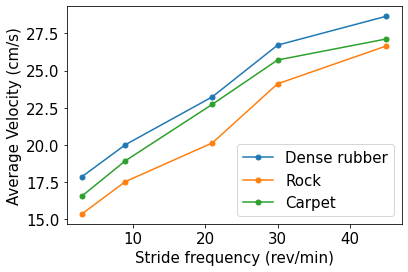
\includegraphics[height=3cm,width=1\textwidth,keepaspectratio]{s_shape_leg/avg_lin_vel_rev_min.png}
        \caption{Средняя линейная скорость робота}
        \label{fig:s_shape_leg/avg_lin_vel_rev_min.png}
    \end{subfigure}

\caption{Пример некоторых входных данных}
\label{fig:example_input}
\end{figure}

% Функция принятия решения для SVM-модели \eqref{eq:SVM}:

% \begin{align}
%     \label{eq:SVM}
%     f(x) = w^T x + b
% \end{align}

% где $x$ --- входной вектор, $w$ является весовым вектором, и $b$ --- смещение.


\begin{figure}[ht!]
    \begin{subfigure}{0.45\textwidth}
        \centering
        \begin{tikzpicture}
            % Include the image in a node
            \node [above right, inner sep=0] (image) at (0,0)
            {\centering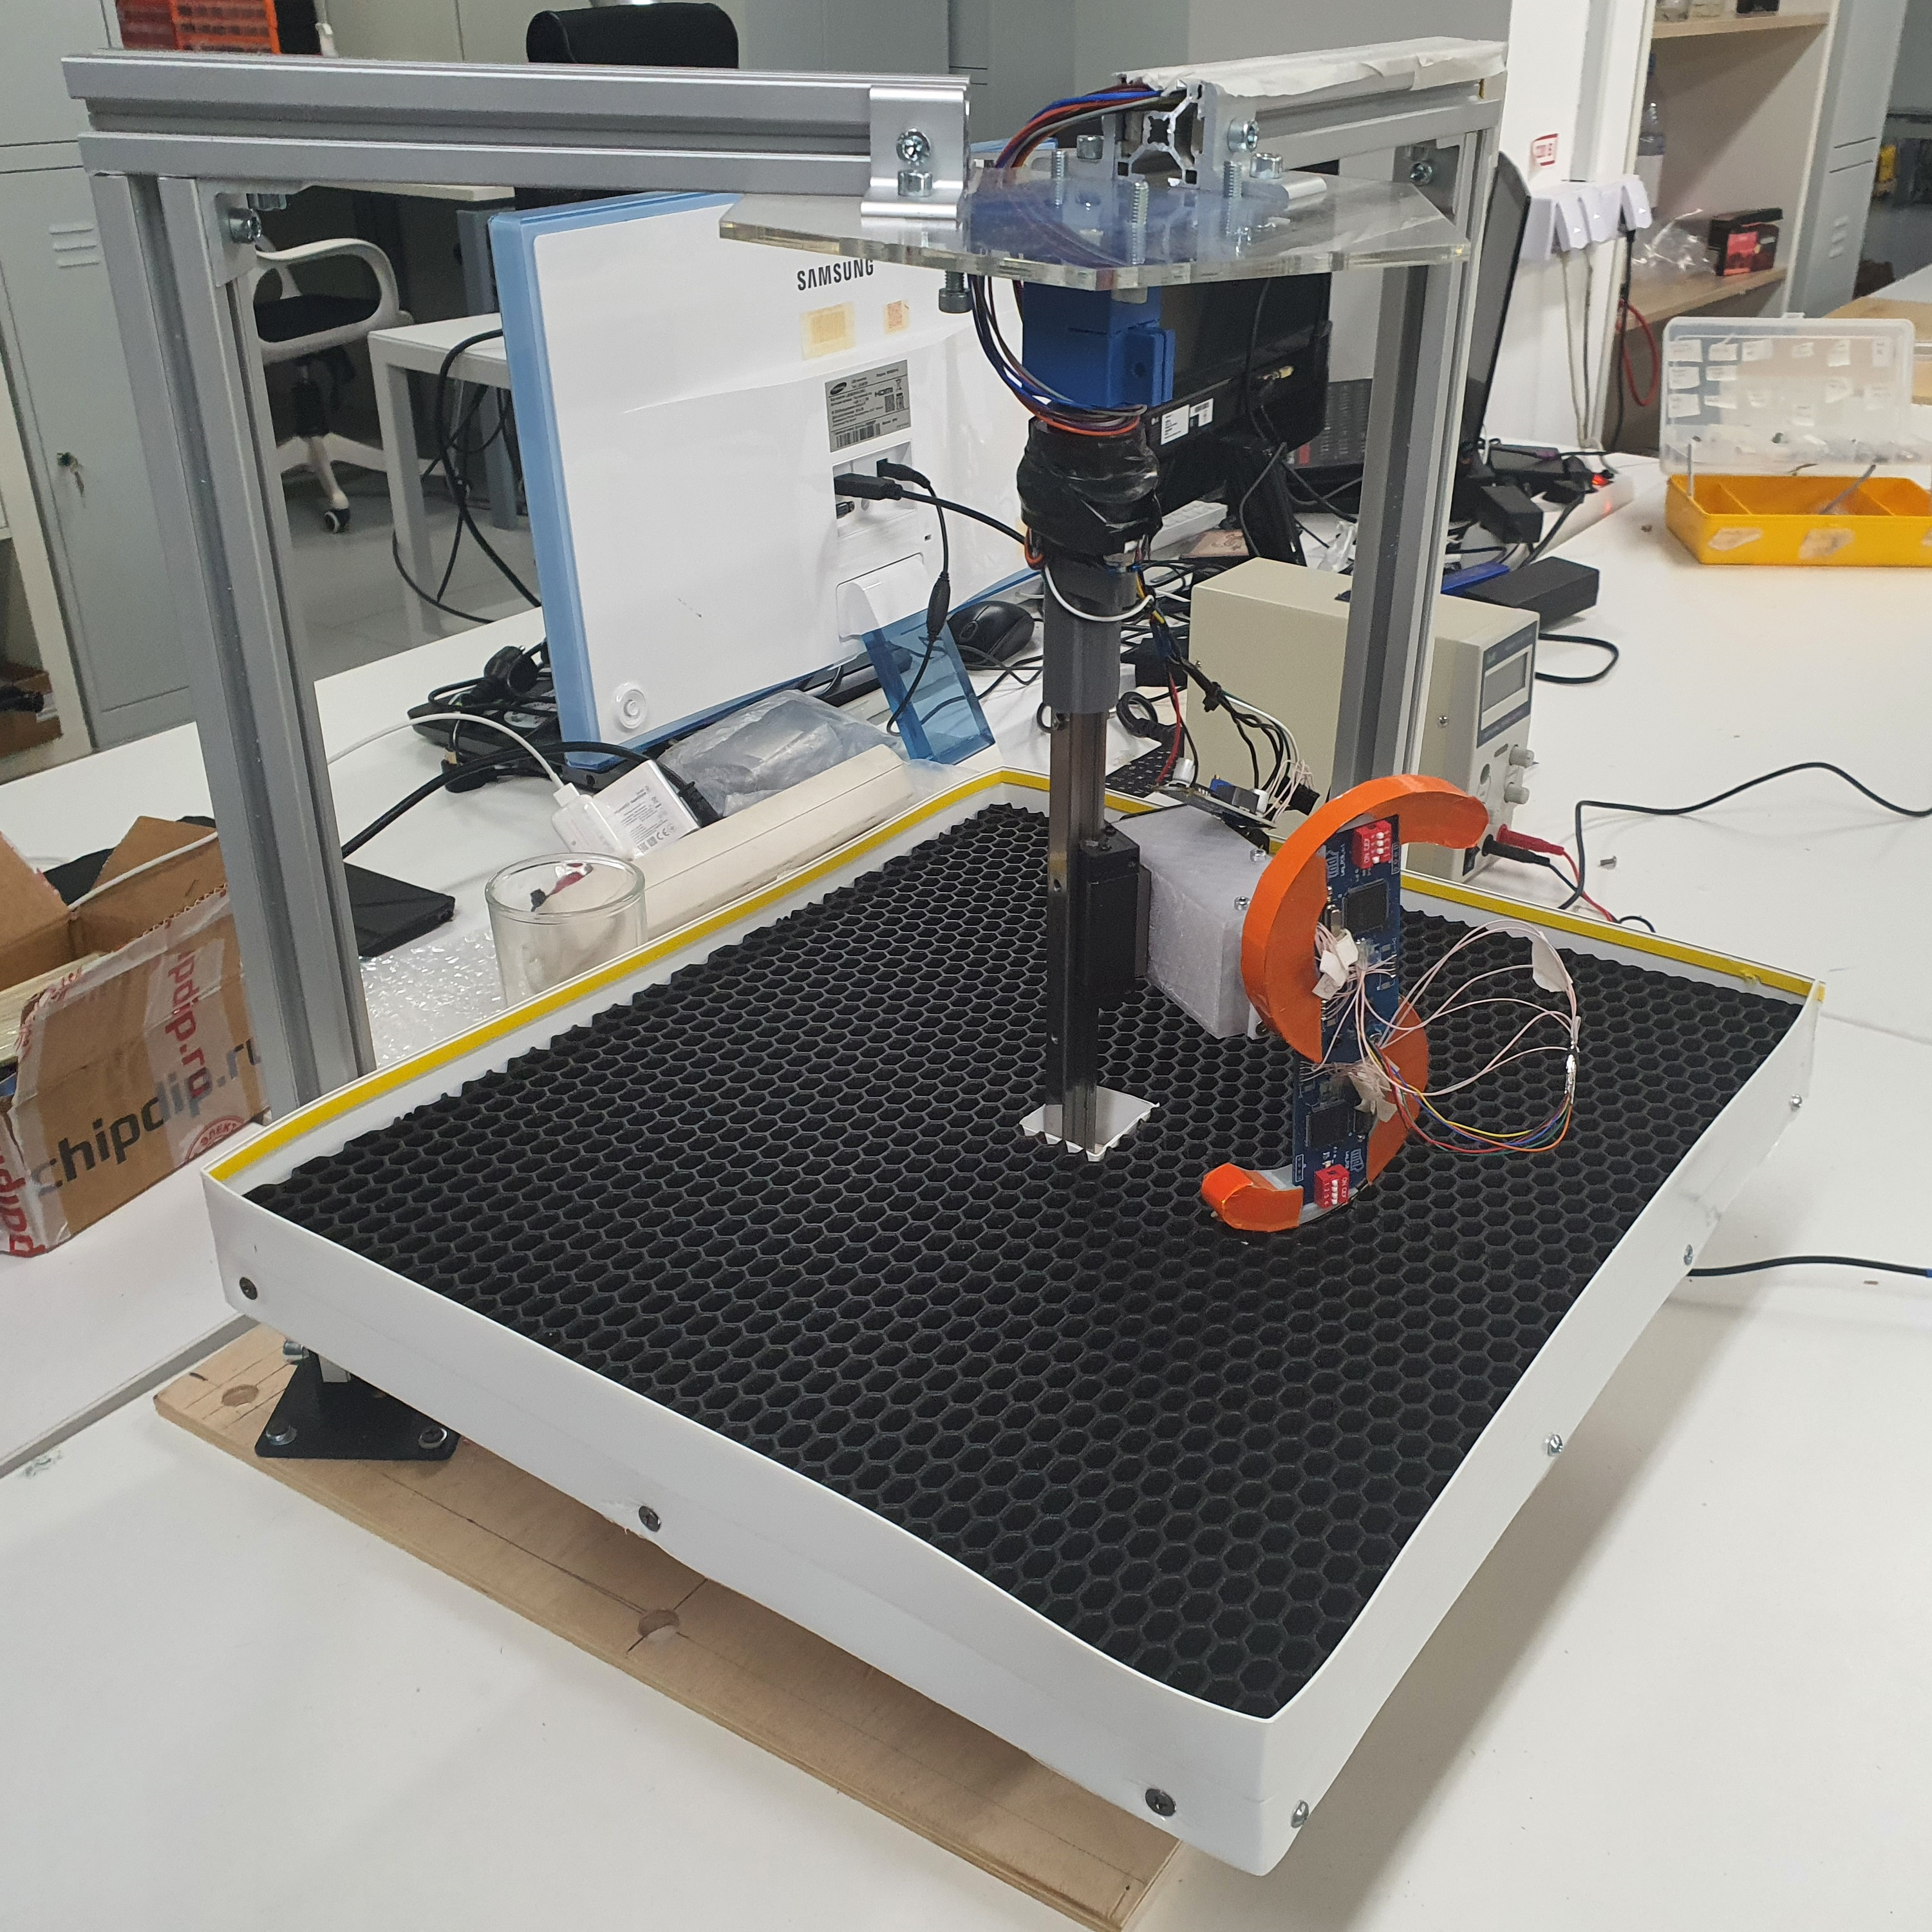
\includegraphics[height=4cm,width=1\textwidth,keepaspectratio]{s_shape_leg/s_leg_setup.JPG}};
            % Create scope with normalized axes
            \begin{scope}[
                x={($ 0.1*(image.south east)$)},
                y={($ 0.1*(image.north west)$)}]
            \draw[stealth-, very thick,green] (3.5,2.5) -- (3,1.5)
            node[rounded corners=3pt,below,black,fill=white]{\tiny Стол для поверхностей};
    
            \draw[stealth-, very thick,green] (7.1,5.4) -- (7.4,7)
            node[rounded corners=3pt,above right,black,fill=white]{\tiny Контроллер};
    
            \draw[very thick,green] (6,6.1) rectangle (8.5,3.5)
            node[above left,black,fill=green]{\tiny S leg};
        \end{scope}
        \end{tikzpicture}
        \caption{Общий вид экспериментальной установки}
    \end{subfigure}
        \begin{subfigure}{0.45\textwidth}
            \centering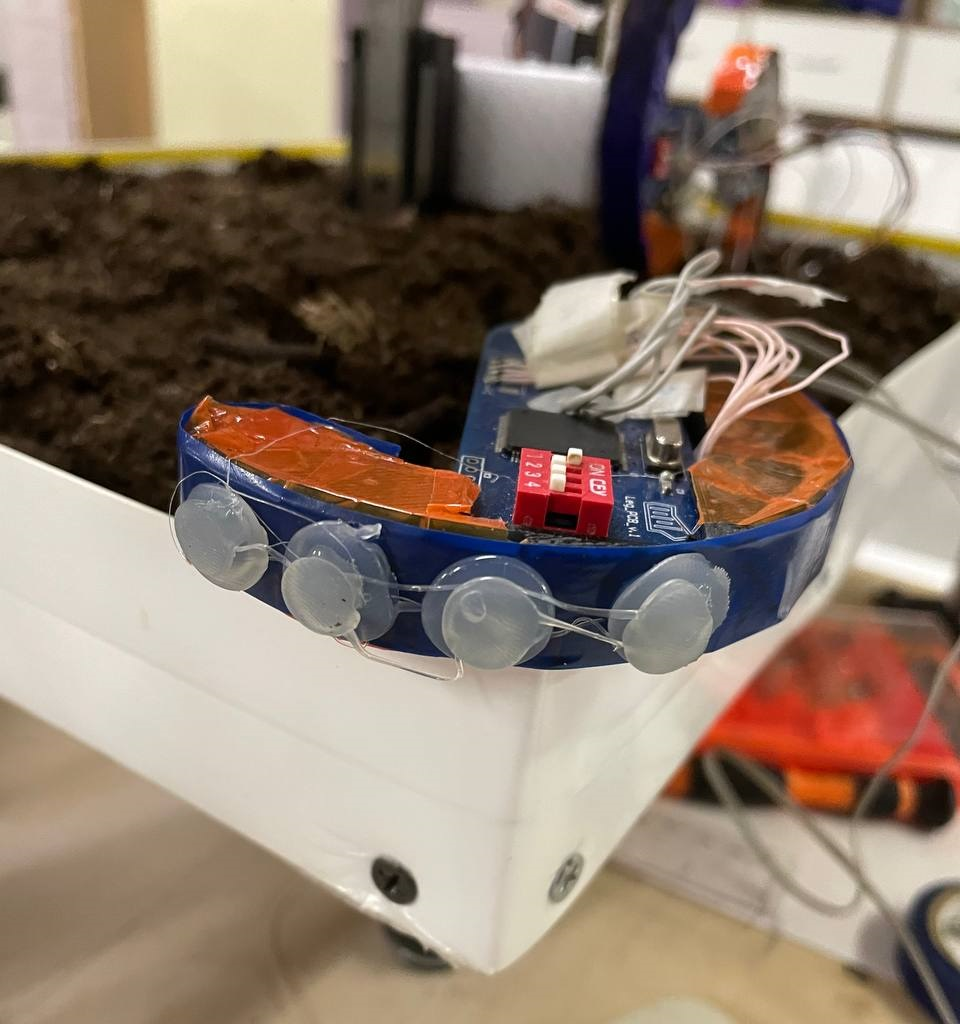
\includegraphics[height=4cm,width=1\textwidth,keepaspectratio]{s_shape_leg/socks_new.jpg}
            \caption{Расположение сенсоров на ноге робота}
            \label{fig:s_shape_leg/socks.jpg}
        \end{subfigure}
        % \begin{subfigure}{0.39\textwidth}
        %     \centering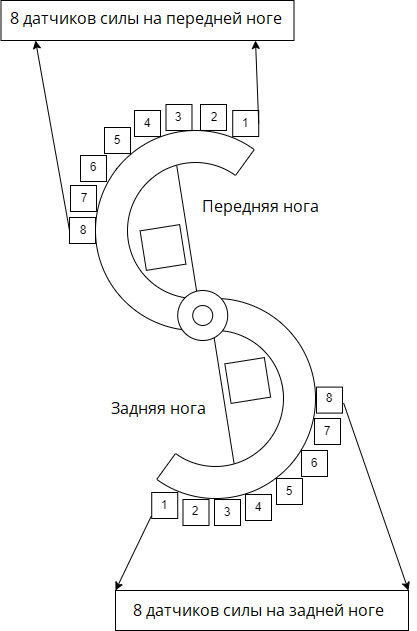
\includegraphics[height=5cm,width=1\textwidth,keepaspectratio]{s_shape_leg/leg_design.png}
        %     \caption{Схематическое расположение сенсоров на ноге установки}
        %     \label{fig:s_shape_leg/leg_design.png}
        % \end{subfigure}

    \caption{Экспериментальная установка}
    \label{fig:s_shape_leg/s_leg_setup.JPG}
\end{figure}

Результат обучения представлен в виде таблицы \tab{tabular:prob_terrain_classification}.

\begin{table}[H]
    \caption{Вероятность определения типа поверхности}
    \label{tabular:prob_terrain_classification}
    \centering
\begin{tabular}{|c|c|c|c|c|} 
    \cline{3-5}
    \multicolumn{1}{l}{} & \multicolumn{1}{l|}{} & \multicolumn{3}{c|}{\textbf{Предсказанный класс}} \\ 
    \cline{3-5}
    \multicolumn{1}{l}{} &  & Камень & Резина & Земля \\ 
    \hline
    \multirow{3}{*}{{\textbf{Истинный класс}}} & Камень & {\cellcolor[rgb]{0.741,0.843,0.929}}84.0\% & 2.56\% & 13.44\% \\ 
    \hhline{|~----|}
     & Резина & 20.1\% & {\cellcolor[rgb]{0.741,0.843,0.929}}67.8\% & 12.1\% \\ 
    \hhline{|~----|}
     & Земля & 1.0\% & 18.9\% & {\cellcolor[rgb]{0.741,0.843,0.929}}80.1\% \\
    \hline
    \end{tabular}
\end{table}

Полученные результаты показывают, что в подавляющем большинстве случаев, удаётся корректно определить класс опорной поверхности. Ошибочные результаты классификации как правило не являются критичными, поскольку определение класса поверхности при движении робота осуществляется многократно в каждой точке касания. И, например, ошибка 20 \% при определении класса означает, что в среднем в каждой пятой точке касания робот будет определять поверхность как более жёсткую, чем она есть на самом деле.

Разработанный метод определения физико-механических свойств поверхности показал достаточно высокий результат классификации поверхностей по трём классам, и может быть применим для более детальной классификации.
